% =====================================================================
%  ARTIGO -- Laboratório de dados do Capítulo 5: pesar corpos centrais
%  Astronomia (AST0001) -- Curso de Física -- UDESC Joinville
%
%  Esqueleto do artigo do laboratório de dados do Capítulo 5, no modelo de
%  artigo da disciplina. O gráfico e a tabela são SEUS: você os produz no
%  Excel ou no Python a partir do arquivo 02_terceira_lei_kepler.csv. Os
%  lugares já estão marcados e referenciados no texto.
%
%  COMO USAR
%   1. Preencha os campos marcados "PREENCHA AQUI".
%   2. Escreva nas seções indicadas, apagando as instruções.
%   3. Compile com pdfLaTeX DUAS vezes (a segunda resolve as referências).
% =====================================================================

\documentclass[10pt,a4paper,twocolumn]{article}

\usepackage[utf8]{inputenc}
\usepackage[T1]{fontenc}
\usepackage[brazil]{babel}
\usepackage{amsmath,amssymb}
\let\Bbbk\relax
\usepackage{newtxtext,newtxmath}
\usepackage{microtype}
\usepackage[a4paper,top=2.4cm,bottom=2.2cm,left=1.9cm,right=1.9cm,
            columnsep=0.7cm]{geometry}
\usepackage{graphicx}
\usepackage{booktabs}
\usepackage{siunitx}
\usepackage{caption}
\usepackage{titlesec}
\usepackage{fancyhdr}
\usepackage{xcolor}
\usepackage[colorlinks=true,linkcolor=udescverde,citecolor=udescverde,
            urlcolor=udescverde]{hyperref}

\definecolor{udescverde}{HTML}{1B6B3A}
\definecolor{cinza}{HTML}{5A5A5A}

\sisetup{output-decimal-marker={,}, per-mode=symbol}

\captionsetup{font=small,labelfont={bf,color=udescverde},labelsep=period}
\titleformat{\section}{\normalfont\bfseries\color{udescverde}}
            {\thesection.}{0.5em}{\MakeUppercase}
\titleformat{\subsection}{\normalfont\bfseries\itshape}{\thesubsection.}{0.5em}{}
\titlespacing*{\section}{0pt}{1.6ex}{0.8ex}
\setlength{\parindent}{1.2em}

% usado pelas tabelas que o laboratório gerou
\newcommand{\compacttables}{\footnotesize\setlength{\tabcolsep}{3pt}}

% ---------------------------------------------------- PREENCHA AQUI
\newcommand{\titulo}{Massas de corpos centrais medidas pela terceira lei de Kepler}
\newcommand{\autores}{PREENCHA: Nome Um, Nome Dois, Nome Três}
% um endereço por autor, na mesma ordem dos nomes
\newcommand{\emails}{aluno1@edu.udesc.br, aluno2@edu.udesc.br, aluno3@edu.udesc.br}
% aparece no cabeçalho das páginas; troquem se preferirem outra forma
\newcommand{\autoresCurto}{PREENCHA: Sobrenome et al.}
\newcommand{\tituloCurto}{Massas pela terceira lei}
\newcommand{\semestre}{2026/2}
% -------------------------------------------------------------------

\pagestyle{fancy}
\fancyhf{}
\fancyhead[L]{\footnotesize\textcolor{cinza}{\autoresCurto}}
\fancyhead[R]{\footnotesize\textcolor{cinza}{\tituloCurto}}
\fancyfoot[C]{\footnotesize\textcolor{cinza}{\thepage}}
\renewcommand{\headrulewidth}{0.3pt}
\fancypagestyle{primeira}{%
  \fancyhf{}\renewcommand{\headrulewidth}{0pt}
  \fancyfoot[C]{\footnotesize\textcolor{cinza}{\thepage}}}

\begin{document}

\twocolumn[
\begin{@twocolumnfalse}

\noindent
\begin{minipage}{0.78\textwidth}
  {\footnotesize\textcolor{udescverde}{\textbf{ASTRONOMIA (AST0001)}}\\[2pt]
   \textcolor{cinza}{Universidade do Estado de Santa Catarina\, $\cdot$\,
   Centro de Ciências Tecnológicas\, $\cdot$\, Curso de Física}\\[2pt]
   \textcolor{cinza}{Joinville, \semestre}}
\end{minipage}
\hfill
\begin{minipage}{0.20\textwidth}
  \raggedleft{
\includegraphics[height=1.5cm]{udesc.png}}
\end{minipage}

\vspace{2pt}
{\color{udescverde}\rule{\textwidth}{1pt}}

\vspace{1.1em}
\begin{center}
  {\LARGE\bfseries \titulo\par}
  \vspace{0.9em}
  {\large \autores\par}
  \vspace{0.3em}
  {\footnotesize\itshape\textcolor{cinza}{\emails}\par}
  \vspace{0.3em}
  {\footnotesize\textcolor{cinza}{Recebido em \today}\par}
\end{center}

\vspace{0.9em}

% ------------------------------------------------------------ RESUMO
% Um parágrafo, de 120 a 200 palavras: contexto em uma frase, o que foi
% feito, que dados, o RESULTADO NUMÉRICO com incerteza, e a conclusão em
% uma frase. Escrito por último, lido primeiro. Sem citar figuras.
\noindent\rule{\textwidth}{0.3pt}
\vspace{0.5em}

{\small
\noindent\textbf{Resumo.}
Escreva aqui, por último. Diga que usou semieixos maiores e períodos de 21
corpos reais, orbitando quatro centros diferentes, e que aplicou a terceira lei
de Kepler na forma newtoniana para pesar cada centro. Apresente as massas
obtidas em números, com incerteza, e compare com os valores tabelados. Diga em
uma frase o que o método mede de fato --- e o que ele não consegue medir.

\vspace{0.6em}
\noindent\textbf{Palavras-chave:} mecânica celeste --- terceira lei de Kepler
--- massas --- órbitas
}

\vspace{0.5em}
\noindent\rule{\textwidth}{0.3pt}
\vspace{1.4em}

\end{@twocolumnfalse}
]
\thispagestyle{primeira}

% =====================================================================
\section{Introdução}
% =====================================================================
% Por que orbitas pesam. A gravidade e a unica interacao que permite medir
% massa a distancia, sem tocar no objeto e sem hipotese sobre o que ele e:
% basta ver algo girar em volta. Diga por que isso importa em astrofisica,
% onde nada pode ser posto em uma balanca.

Escreva aqui.

% =====================================================================
\section{Revisão Teórica}
% =====================================================================
% A equacao, e as hipoteses que ela carrega.

A terceira lei de Kepler, na forma que a gravitação newtoniana produz, é uma
balança gravitacional:
\begin{equation}
P^{2} = \frac{4\pi^{2}a^{3}}{G\,(M_1+M_2)} ,
\qquad\text{ou}\qquad
M = \frac{4\pi^{2}a^{3}}{G\,P^{2}} .
\label{eq:kepler3}
\end{equation}
Em unidades astronômicas, anos e massas solares, os fatores desaparecem e ela
vira $M = a^{3}/P^{2}$.
% ATENCAO -- diga isto em voz alta no texto:
%  (a) a lei traz a SOMA das massas, nao a massa central. A aproximacao
%      M = a^3/P^2 supoe m << M. Estime o erro que ela introduz para as luas
%      galileanas, onde a razao de massas e maior.
%  (b) a e o semieixo maior da orbita RELATIVA.
%  (c) a excentricidade nao aparece: orbitas alongadas e circulares de mesmo
%      a tem o mesmo periodo.

% =====================================================================
\section{Dados e Método}
% =====================================================================

Escreva aqui: qual arquivo, quantos corpos, quantos centros, e como você
agrupou. Diga também como obteve a incerteza de cada massa --- a dispersão
entre os corpos de um mesmo grupo é uma estimativa honesta.

% =====================================================================
\section{Resultados}
% =====================================================================

\begin{figure}[t]
\centering
% troque pelo SEU grafico
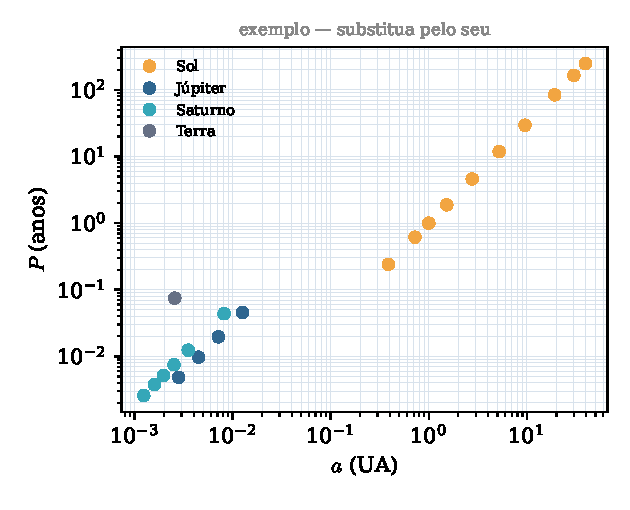
\includegraphics[width=\columnwidth]{figuras/log_p_log_a.pdf}
\caption{$\log P$ contra $\log a$ para os 21 corpos, com um símbolo por
sistema. As retas têm todas inclinação $3/2$ --- é a terceira lei. O que muda
de um sistema para outro é o \textbf{coeficiente linear}, e é ele que carrega
a massa do corpo central.}
\label{fig:loglog}
\end{figure}

\begin{table}[t]
\centering\footnotesize
\caption{Massas centrais obtidas de $M=a^{3}/P^{2}$, em massas solares e em
quilogramas, com os valores tabelados para comparação.}
\label{tab:massas}
\begin{tabular}{lrrrr}
\toprule
centro & $n$ & $M$ ($M_\odot$) & $M$ (kg) & tabelado (kg) \\
\midrule
Sol      &  &  &  & $1{,}989\times10^{30}$ \\
Júpiter  &  &  &  & $1{,}898\times10^{27}$ \\
Saturno  &  &  &  & $5{,}683\times10^{26}$ \\
Terra    &  &  &  & $5{,}972\times10^{24}$ \\
\bottomrule
\end{tabular}
\end{table}

Escreva aqui, apoiando-se na Figura~\ref{fig:loglog} e na
Tabela~\ref{tab:massas}.

% =====================================================================
\section{Discussão}
% =====================================================================
% Tres coisas que este laboratorio cobra:
%
%  (a) Por que as retas do grafico sao PARALELAS mas deslocadas? Traduza o
%      deslocamento vertical em massa, e mostre a conta.
%
%  (b) A Terra aparece com UM unico satelite. Uma media de um valor so nao
%      tem incerteza estatistica. Diga o que isso significa para aquela linha
%      da tabela, e o que seria preciso para melhora-la.
%
%  (c) O que este metodo NAO mede. Ele da a soma das massas do sistema, e da
%      apenas isso: nao separa as duas, nao diz do que o corpo e feito, nao
%      distingue uma estrela de um buraco negro de mesma massa. Diga onde
%      essa limitacao passa a importar.

Escreva aqui.

% =====================================================================
\section{Conclusão}
% =====================================================================
% Tres a cinco frases: o que foi medido, com que numeros, e o que a
% concordancia (ou a falta dela) com os valores tabelados demonstra.

Escreva aqui.

% =====================================================================
\section*{Referências}
% =====================================================================

\begin{thebibliography}{9}\footnotesize
\bibitem{apostila} LIMA, R. C. R. \emph{Astrofísica Moderna: apostila de
capítulos de estudo}. UDESC Joinville, 2026. Capítulo 5.
\bibitem{co} CARROLL, B. W.; OSTLIE, D. A. \emph{An Introduction to Modern
Astrophysics}. 2. ed. Cambridge University Press, 2017.
\bibitem{jpl} PREENCHA: a fonte dos valores tabelados de massa.
\end{thebibliography}

\end{document}
